\documentclass[referee,a4paper,12pt]{swsc}

\usepackage{graphicx}
\usepackage{txfonts}
\usepackage{subfigure}
\usepackage{epstopdf}
\usepackage{lineno}
\usepackage[authoryear,round]{natbib}
\usepackage[backref]{hyperref}
\usepackage{url}
\usepackage{longtable}
\bibliographystyle{plainnat}
\hypersetup{colorlinks=true,citecolor=cyan,urlcolor=cyan,linkcolor=blue}

\author{Andrew Leonard*
        \and Huw Morgan}

\institute{Institute of Mathematics, Physics and Computer Science, Aberystwyth University, Ceredigion, SY23 3BZ, Wales\\
					 \email{\href{mailto:ajl7@aber.ac.uk}{ajl7@aber.ac.uk}}}

\title{Using temperature distributions of active regions to investigate flare activity}

\begin{document}

\begin{linenumbers}

\titlerunning{Temperature distributions of active regions}
\authorrunning{Leonard and Morgan}

\abstract
	{}
	{We aim to investigate whether signatures of solar flares can be seen in the temperature distributions of flaring active regions before the flares occur. Such a signature, if found, might form the basis of a flare prediction algorithm.}
	{A recently developed and extremely fast temperature-mapping method is used to determine the temperature of flaring active regions. This process is repeated for the 30 minutes preceding a flare at 1-minute intervals. How the distribution of temperatures changes in each active region during this time is compared in order to investigate whether or not there is any repeatable pattern which may indicate that a flare is about to occur.}
	{We find that with the current sample size and within the 30 minutes before flare onset, there is no clear signature of flare occurance in active region temperature distributions. However, for the majority of M and X class flares studied, the mean temperatures of the active regions remained below the mean temperature at the flare onset time for much of the preceding 30 minutes. This should be investigated further with a larger sample of M and X class flares.}
	{}

\maketitle

%===========================================================================
\section{Introduction}
Solar flares are a complicated and as yet not fully understood phenomenon.
In particular, growing emphasis has been placed in recent years on studying how to predict when a flare will occur, since flares and associated coronal phenomena can have significant detrimental effects on a variety of modern electronic infrastructure. % This needs some work, but I'm not sure how it needs to change. Possibly add a reference?
Many studies have been devoted to the topic of flare prediction (eg, \citealt{Korsos2014, Ahmed2011, Bloomfield2012}, etc.), but few have looked at the temperature of the active regions associated with flares before the flare occurs. % Possibly cite more papers or a review. Bit more description on lack of temperature studies

Studies of coronal temperatures date back several decades. % Stick some references here to early DEM studies
However, the Atmospheric Imaging Assembly (AIA; \cite{Lemen2011}) which began observing the Sun in 2010 allows unprecedented access to observations with very high spatial and temporal resolution.
This allows investigation of temperature distributions on small spatial scales with high cadence. % Don't much like this sentence, but oh well
The six Fe-based EUV channels of AIA also provide greater constraints on temperature than previous coronal imagers \citep{Guennou2012, Guennou2012a}.

This work makes use of the capabilities of AIA in order to investigate the temperature distributions of several flaring active regions.
The aim is to search for a common signature of flare activity in these temperature distributions before flares occur, which, if found, could form the basis of a flare prediction algorithm.

%===========================================================================
\section{Method}
This investigation looks at temperature distributions of active regions over the 30 minutes before a flare occurs.
We also directly compare the temperatures of the corresponding active regions at several different times before the flares.

Although it is faster than others of its kind, the temperature-calculating method used here requires a very large amount of AIA data, which can take a long time to download and process.
As such this work investigates only a relatively small number of flares and the results should not be considered definitive.
Rather they are a proof of concept; they demonstrate the type of study made available by fast temperature analysis of the corona, which has only been made possible by the high-quality data provided by AIA.

\subsection{Temperature analysis}
The core of this analysis is the temperature map method described by \cite{Leonard} (henceforth Paper I). \defcitealias{Leonard}{Paper I}
Briefly, this method compares the relative brightnesses in each AIA wavelength channel at a given time and infers the best-fitting temperature from that comparison. % This can be phrased more descriptively
This allows the temperature of the corona to be estimated for every pixel of an AIA image, resulting in very high resolution temperature maps.
Crucially, this method produces temperature maps extremely quickly, which allows us to investigate coronal temperatures during localised dynamic events such as flares.
With other, slower methods, such studies are infeasible due to the computation time required.
An example temperature map is shown in Figure \ref{fig:example_tmap}.

The \citetalias{Leonard} method also allows easy `tracking' of solar regions by cropping the temperature map around a given pair of Carrington heliographic coordinates, which rotate at approximately the rate of solar rotation.
This tracking is demonstrated in Figures \ref{fig:trackdemo1} and \ref{fig:trackdemo2}, each of which shows a cropped region of an AIA 17.1nm image containing active region AR11158, the corresponding temperature map and a larger 17.1nm image showing the location of the region in the corona.
Note that the small, bright loops in the centre of the active region are highlighted in red, indicating temperatures of up to $log(T) \sim 6.3$, while some larger, fainter loops around the edges are at temperatures of around $log(T) \sim 6.15$.
These temperatures are consistant with values found by other authors for active region loops. % Reference the shit out of that comment.

\begin{figure}
	\centering
		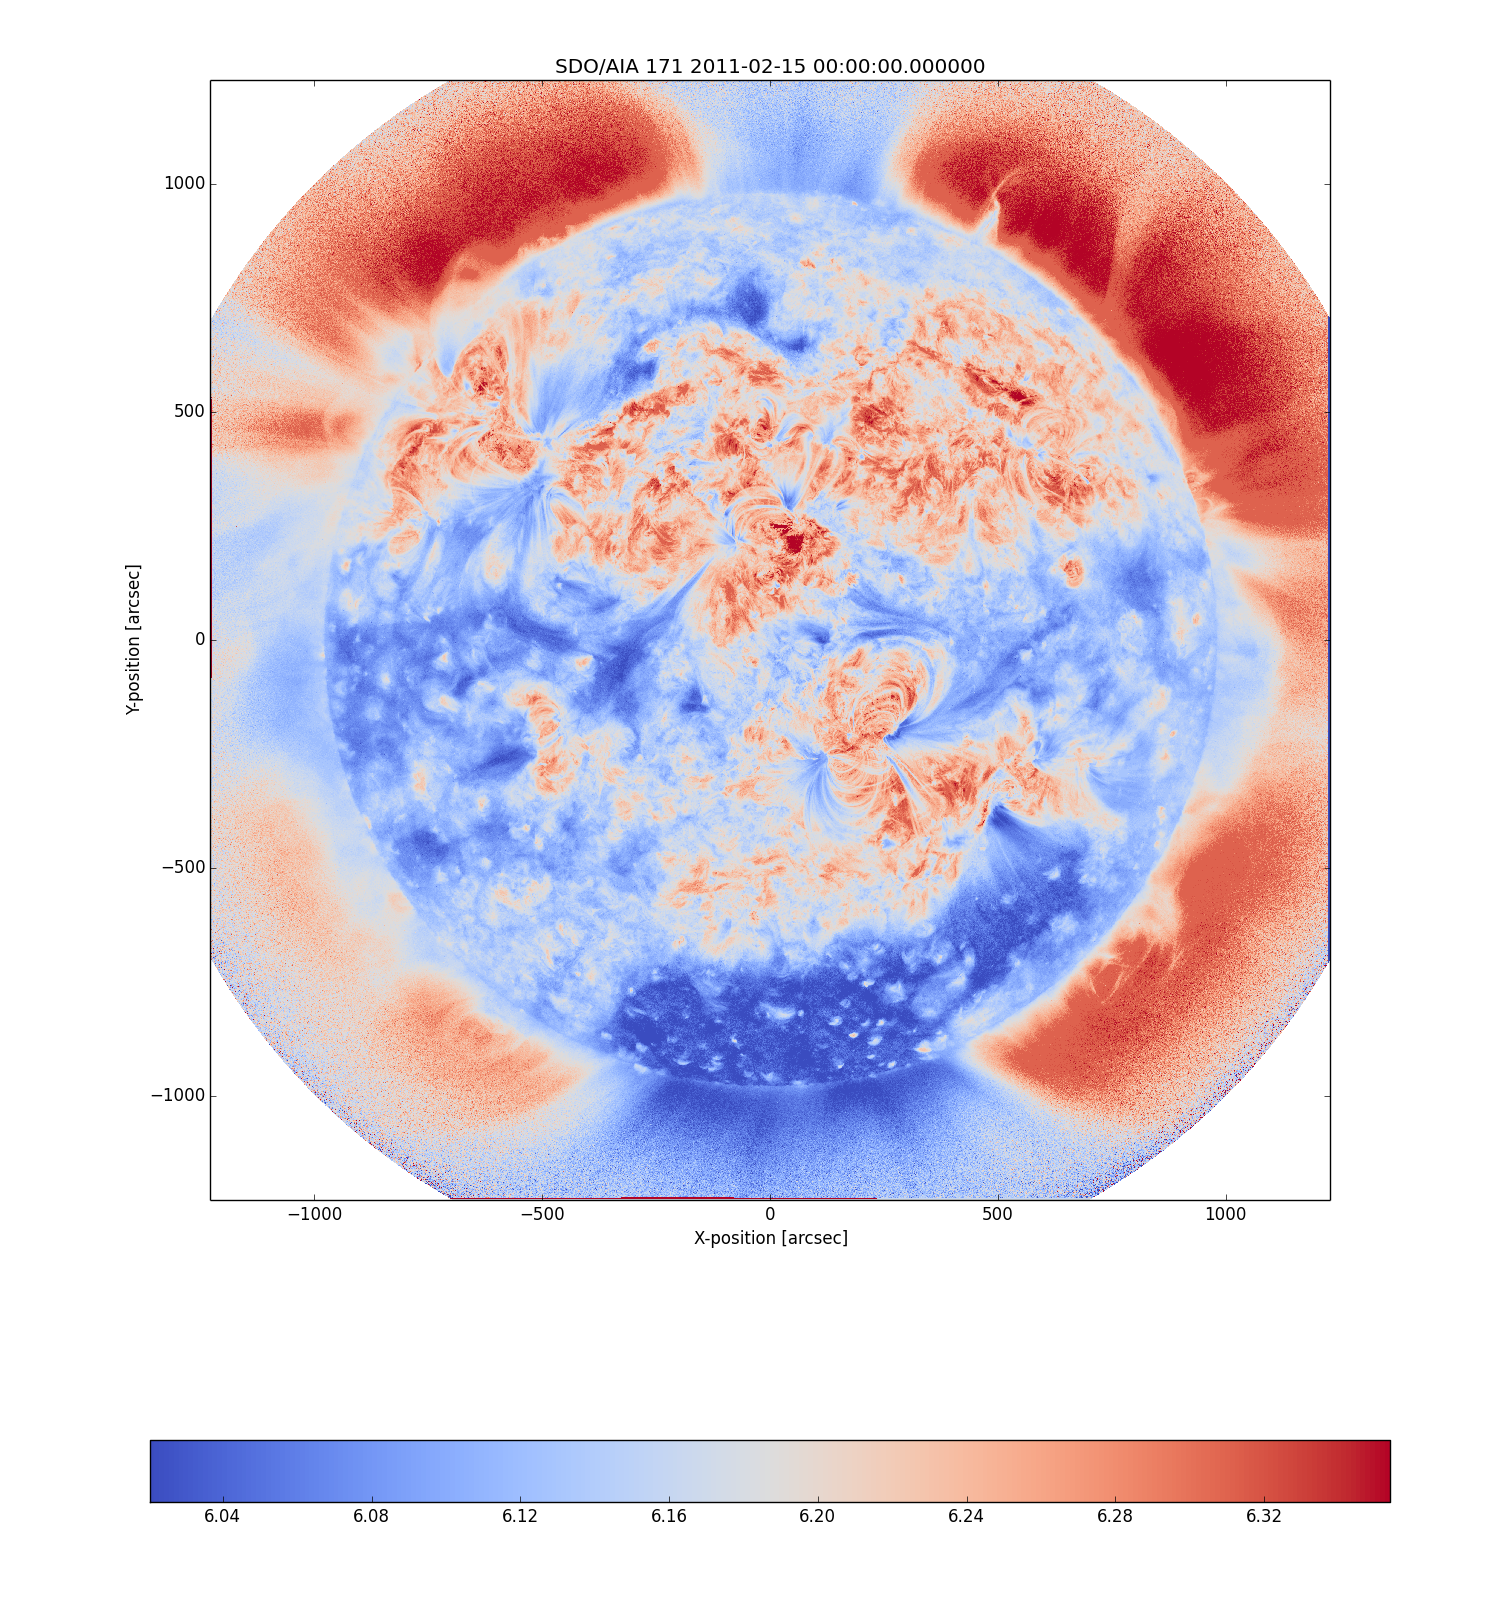
\includegraphics[width=\columnwidth]{2011-02-15T00_00_00.png}
	\caption{Example temperature map for the full solar corona at 2011-02-15 00:00. Temperatures are displayed on a logarithmic scale.}
	\label{fig:example_tmap}
\end{figure}

\begin{figure}
	\centering
		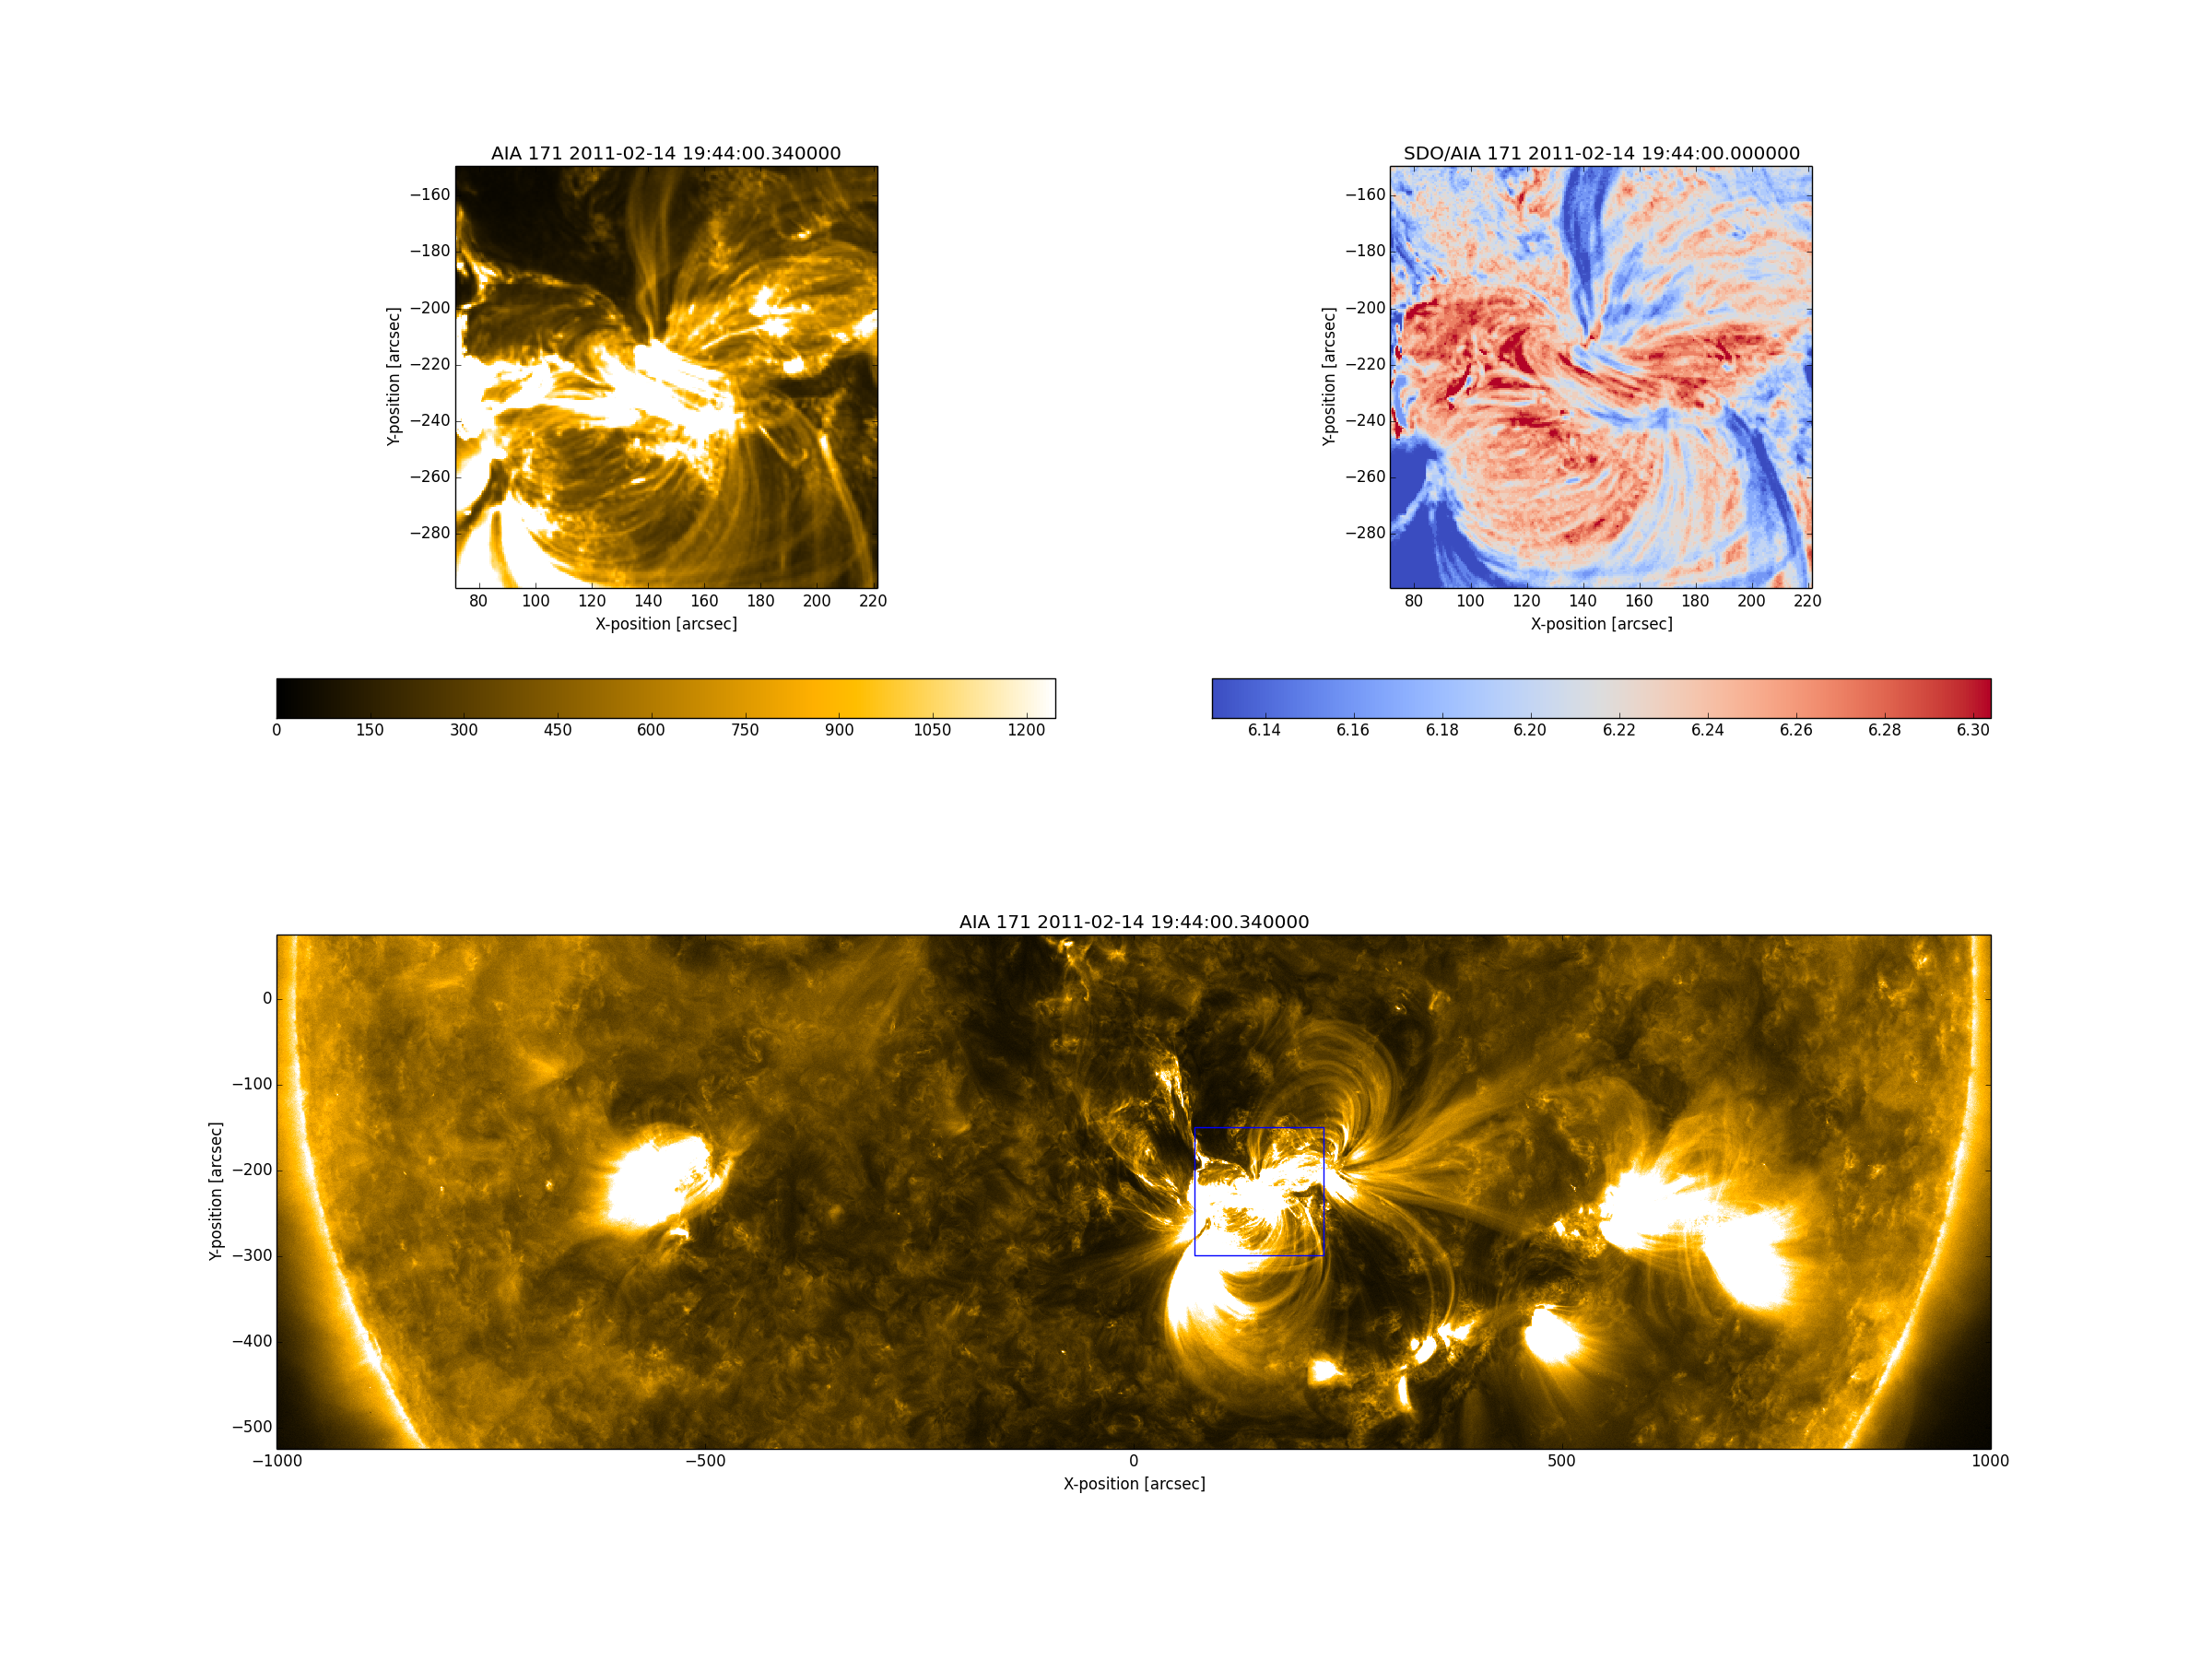
\includegraphics[width=0.9\columnwidth]{20110214T194400with171.png}
	\caption{Top left: Cropped 17.1nm AIA image showing active region AR 11158 at 2011-02-14 19:44:00. Top right: temperature map of active region AR11158 at 2011-02-14 19:44:00. Bottom: Larger 17.1nm image; the blue square outlines the region shown in the top images.}
	\label{fig:trackdemo1}
\end{figure}
\begin{figure}
	\centering
		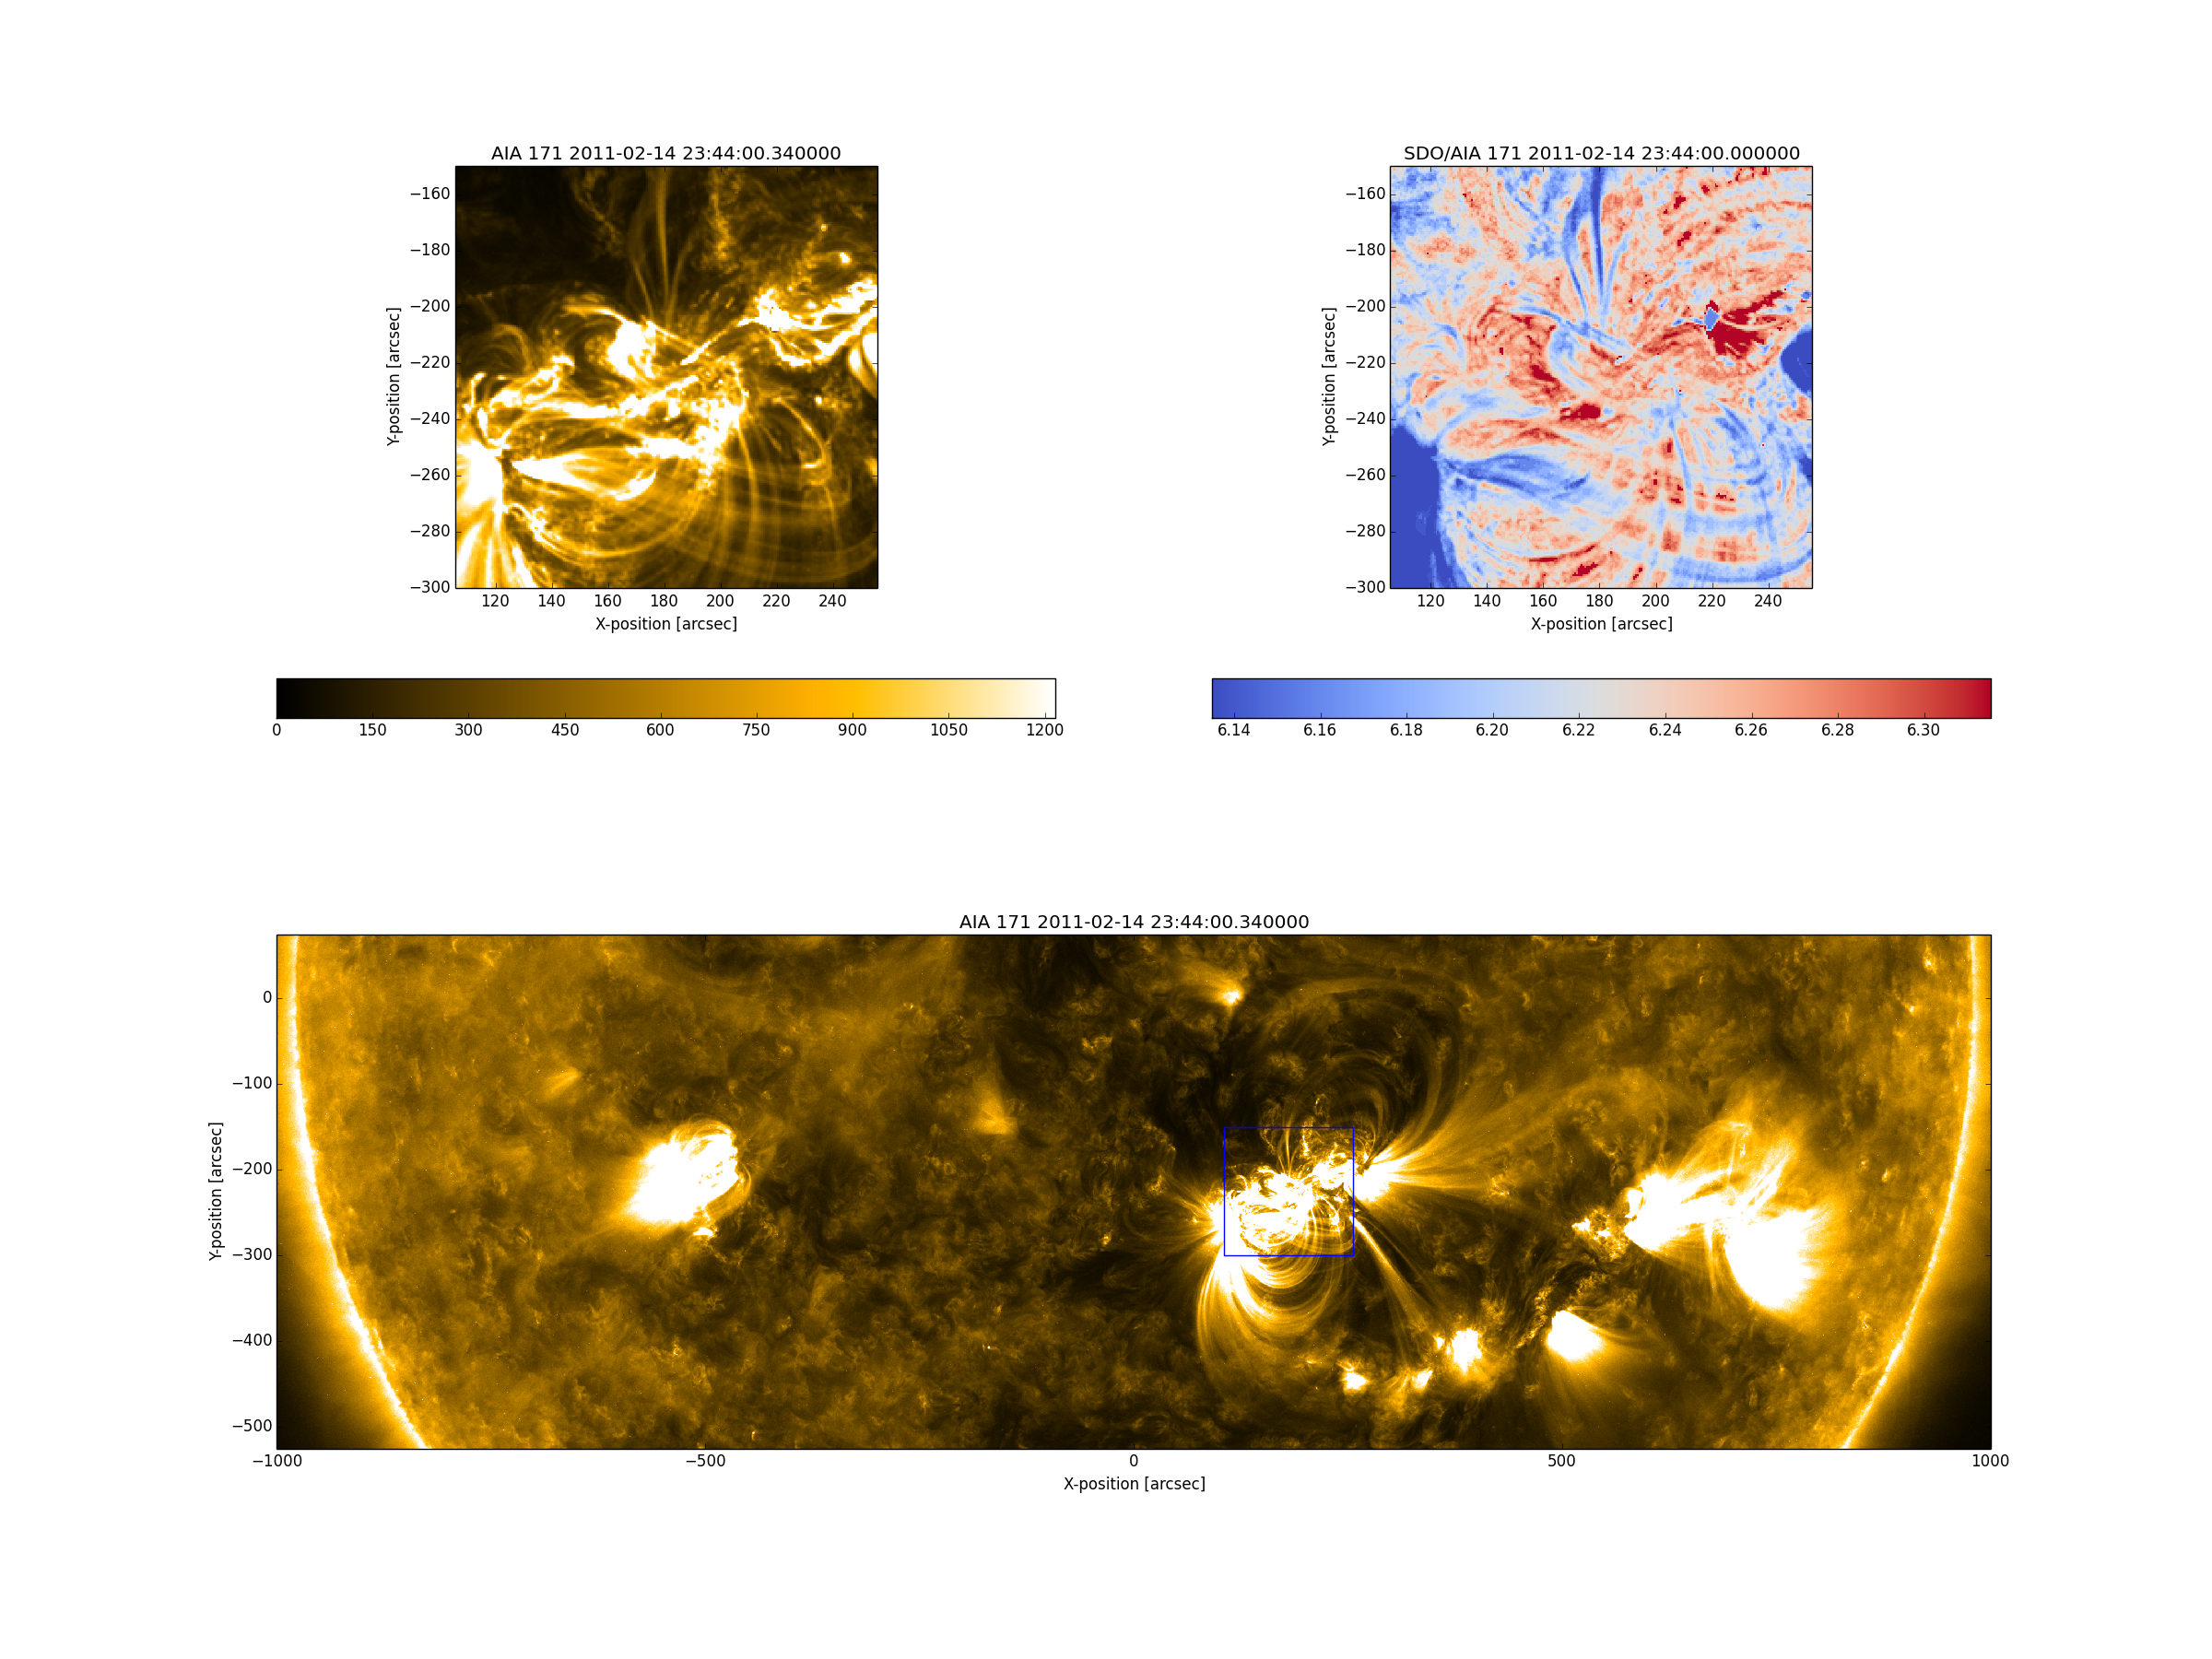
\includegraphics[width=0.9\columnwidth]{20110214T234400with171.png}
	\caption{The same images as Figure \ref{fig:trackdemo1} for time 2011-02-14 23:44:00.}
	\label{fig:trackdemo2}
\end{figure}

\subsection{Active region analysis}
The temperature map method described in \citetalias{Leonard} was used to investigate the temperatures of the active regions associated with flares which occured during February and March 2011.
These months were chosen because several flares occured during this time with a wide range of peak fluxes.
The flares detected included many small flares (B and C class) as well as several larger M class flares and two X class flares.

For each flare event investigated, a temperature map was calculated for a 150 x 150 arcsec area around the corresponding active region at 1-minute intervals for the 30 minutes preceding the start of the flare.
The maximum, 95th percentile, mean, 5th percentile and minimum temperatures were then calculated for each temperature map for each flare in order to compare if and how the bulk temperature of the active regions changed before the flare.
The 95th and 5th percentiles were calculated because the maximum and minimum may be affected by small numbers of unusually high or low temperature pixels, which may not accurately represent how the bulk temperature of the active region changes with time. % Decide if it's worth doing min and max as well as percentiles
Each of these parameters was plotted against time for each active region, and was compared to the peak flux of the flares for all active regions.

The start times of the flares and the locations of the active regions on the solar disk were obtained by querying the Heliophysics Events Knowledgebase (HEK), a database of solar features and events. % Consider putting more detail here
The specific flares investigated are listed in Table \ref{tab:flares} along with the active region associated with each.
Note that not all flares occuring in this time were studied, since for some flares the neccessary AIA data were not available to temperature map the full 30-minute range before the flare onset.
Flares with missing data were excluded from the study.

%===========================================================================
\section{Results}
\subsection{Temperature change over time} \label{sec:temps_v_time}
Figures \ref{fig:allars_max} - \ref{fig:allars_mean} show how the temperature properties of the active region changed during the 30 minutes preceding each flare.
All of the flares studied are plotted in each of these figures so that any changes common to many flares can be easily noticed.
The maximum, 95th percentile and mean temperatures are plotted in figures \ref{fig:allars_max}, \ref{fig:allars_p95} and \ref{fig:allars_mean} respectively.
In each figure, B, C, M and X class flares are plotted separately in the panels from left to right respectively.

% Description of plots for maximum
From the plots in Figure \ref{fig:allars_max} it can be seen that the maximum temperature of each active region varies significantly, with no clear increase or decrease at any particular time before the flare.
This is the case for both small and large flares.
However, it is perhaps interesting to note that many of the active regions associated with C class flares show temperature spikes which reach much higher temperatures than other ARs studied, even those associated with larger flares.

% Description of plots for 95
The 95th percentile temperature (Figure \ref{fig:allars_p95}) is much more stable than the maximum for the active regions studied, staying fairly constant within a small range of temperatures well below the typical maximum temperatures.
Again, active regions associated with C class flares show slightly more variation in temperature than others.
However, there is still no clear indication of any trend of temperature before flares.

% Description of plots for mean
The plots of active region mean temperature in Figure \ref{fig:allars_mean} show that the temperature of each individual active region varies very little over time, but that the temperature can vary quite a bit from one active region to another.
The top left plot of Figure \ref{fig:allars_mean} shows that the active region which produced the one X class flare studied does have a higher mean temperature than those which produced M class flares throughout the time interval.
However, it is still cooler than several of the B and C class flare active regions.
The bottom right plot shows that the active regions of the M and X class tend to stay below the temperature at the flare start time, though only by a very small amount and not in all cases.

% Description of results for p5 and min
The 5th-percentile and minimum values of the temperature maps showed very little variation for all active regions.
The 5th-percentile temperature was either log(T) = 5.85 or log(T) = 6.16 for all regions, with a few switching between the two values during the 30-minute period.
Similarly, the minimum temperature of all active regions was either log(T) = 5.79, log(T) = 5.80 or log(T) = 5.85 throughout the pre-flare period.
These temperatures showed no variation with the class of the associated flare.
Plots of these results are not shown here.

% X-flare lines should be darker on all these plots
\begin{figure}
	\centering
		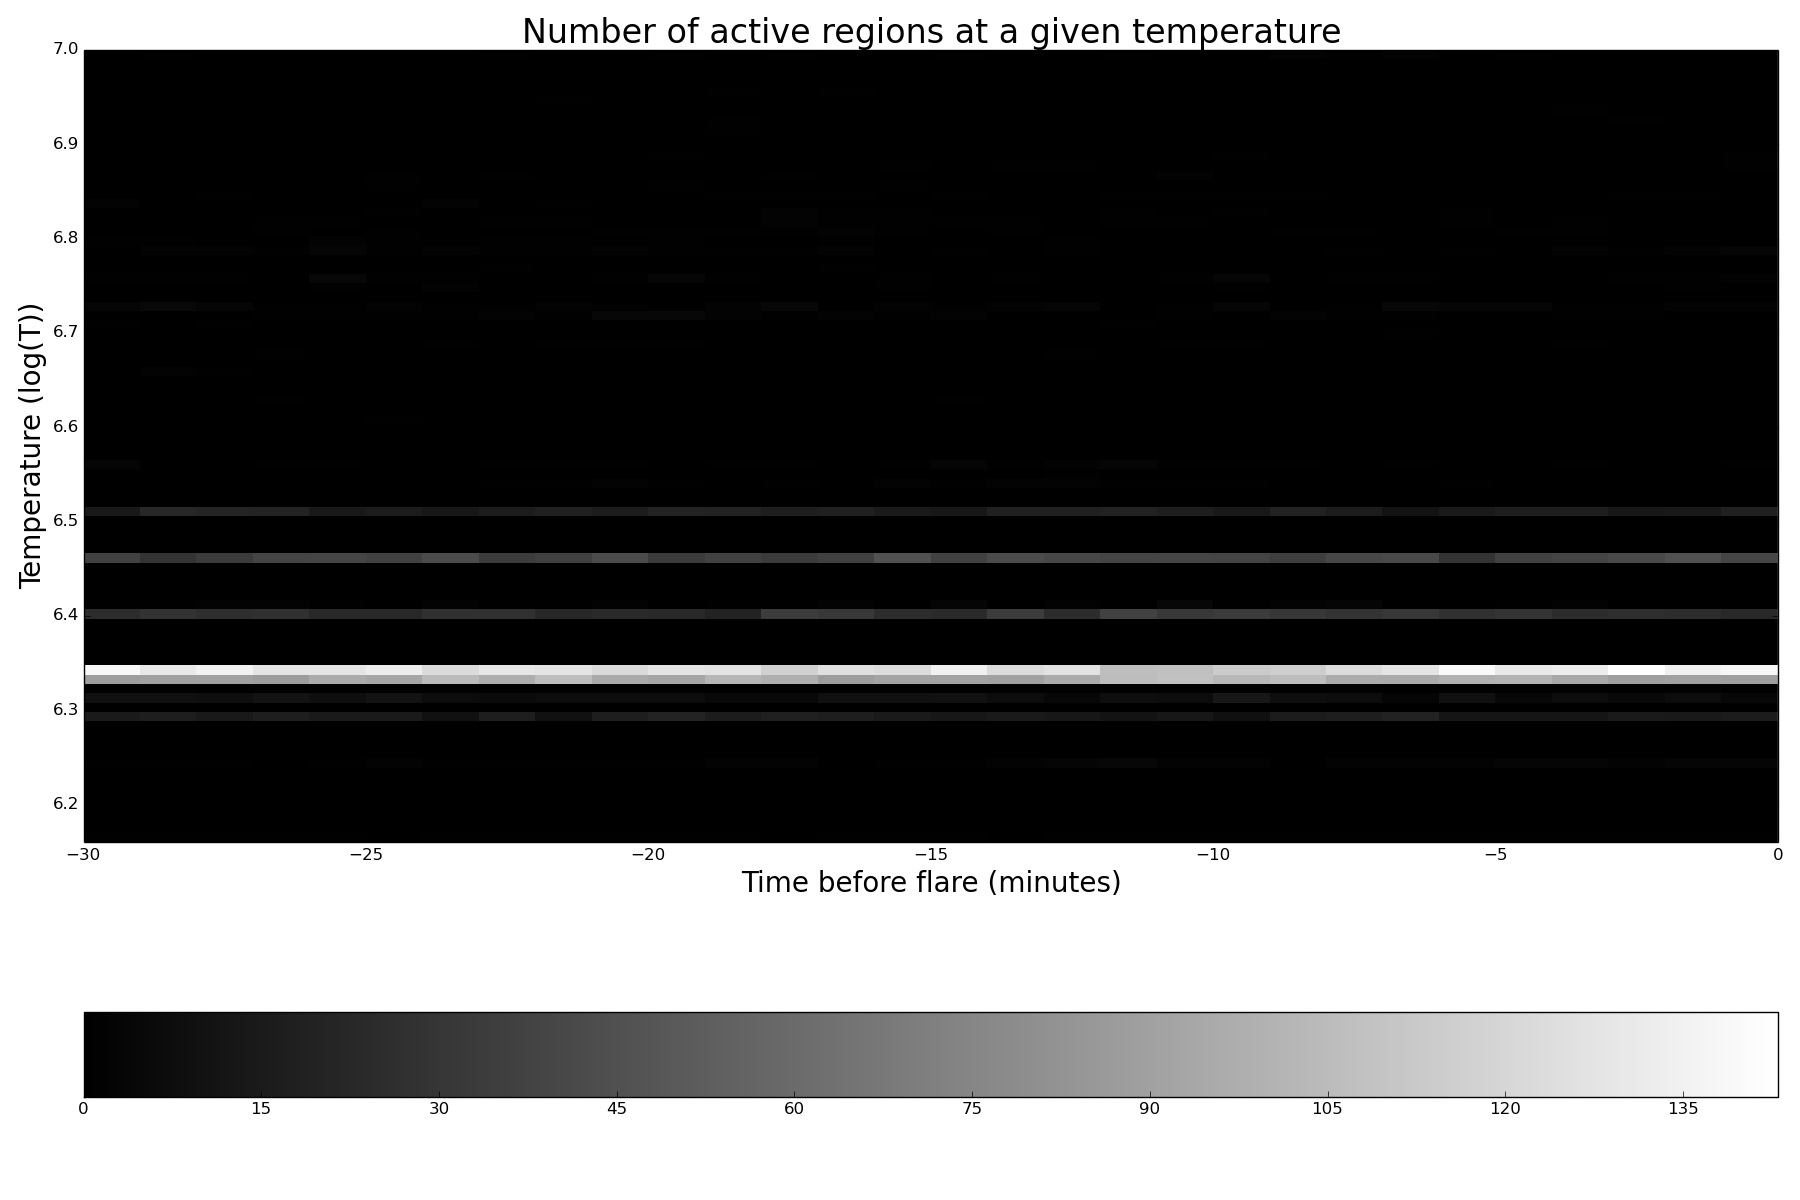
\includegraphics[width=\columnwidth]{tempplotsmax/allars_hist.png}
	\caption{Change in maximum temperature of the corresponding active region plotted for each flare as a function of time before the flare began.
		Flares are separated by class, with flare peak flux increasing from left to right.}
	\label{fig:allars_max}
\end{figure}
\begin{figure}
	\centering
		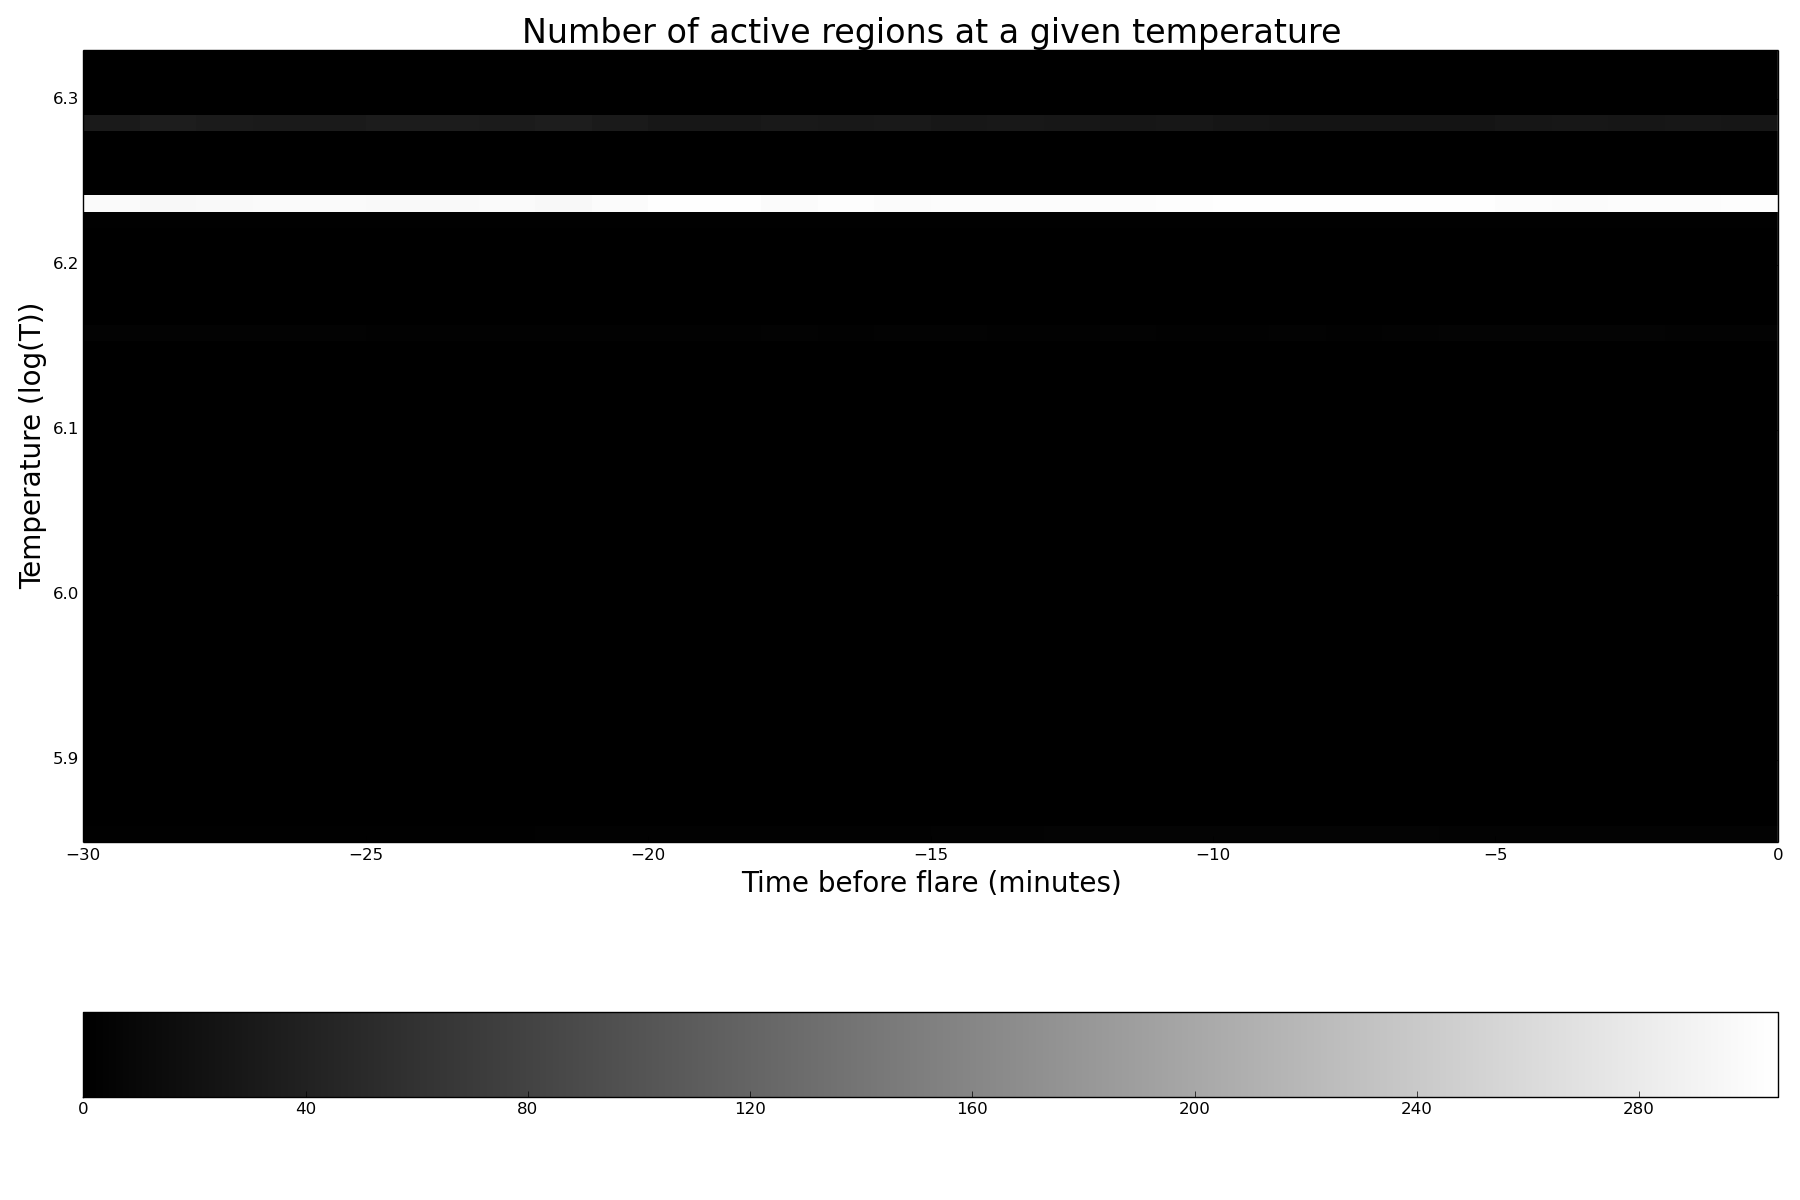
\includegraphics[width=\columnwidth]{tempplots_p95/allars_hist.png}
	\caption{Change in 95th percentile temperature of the corresponding active region plotted for each flare as a function of time before the flare began.
		Plots are the same as in Figure \ref{fig:allars_max}.}
	\label{fig:allars_p95}
\end{figure}
\begin{figure}
	\centering
		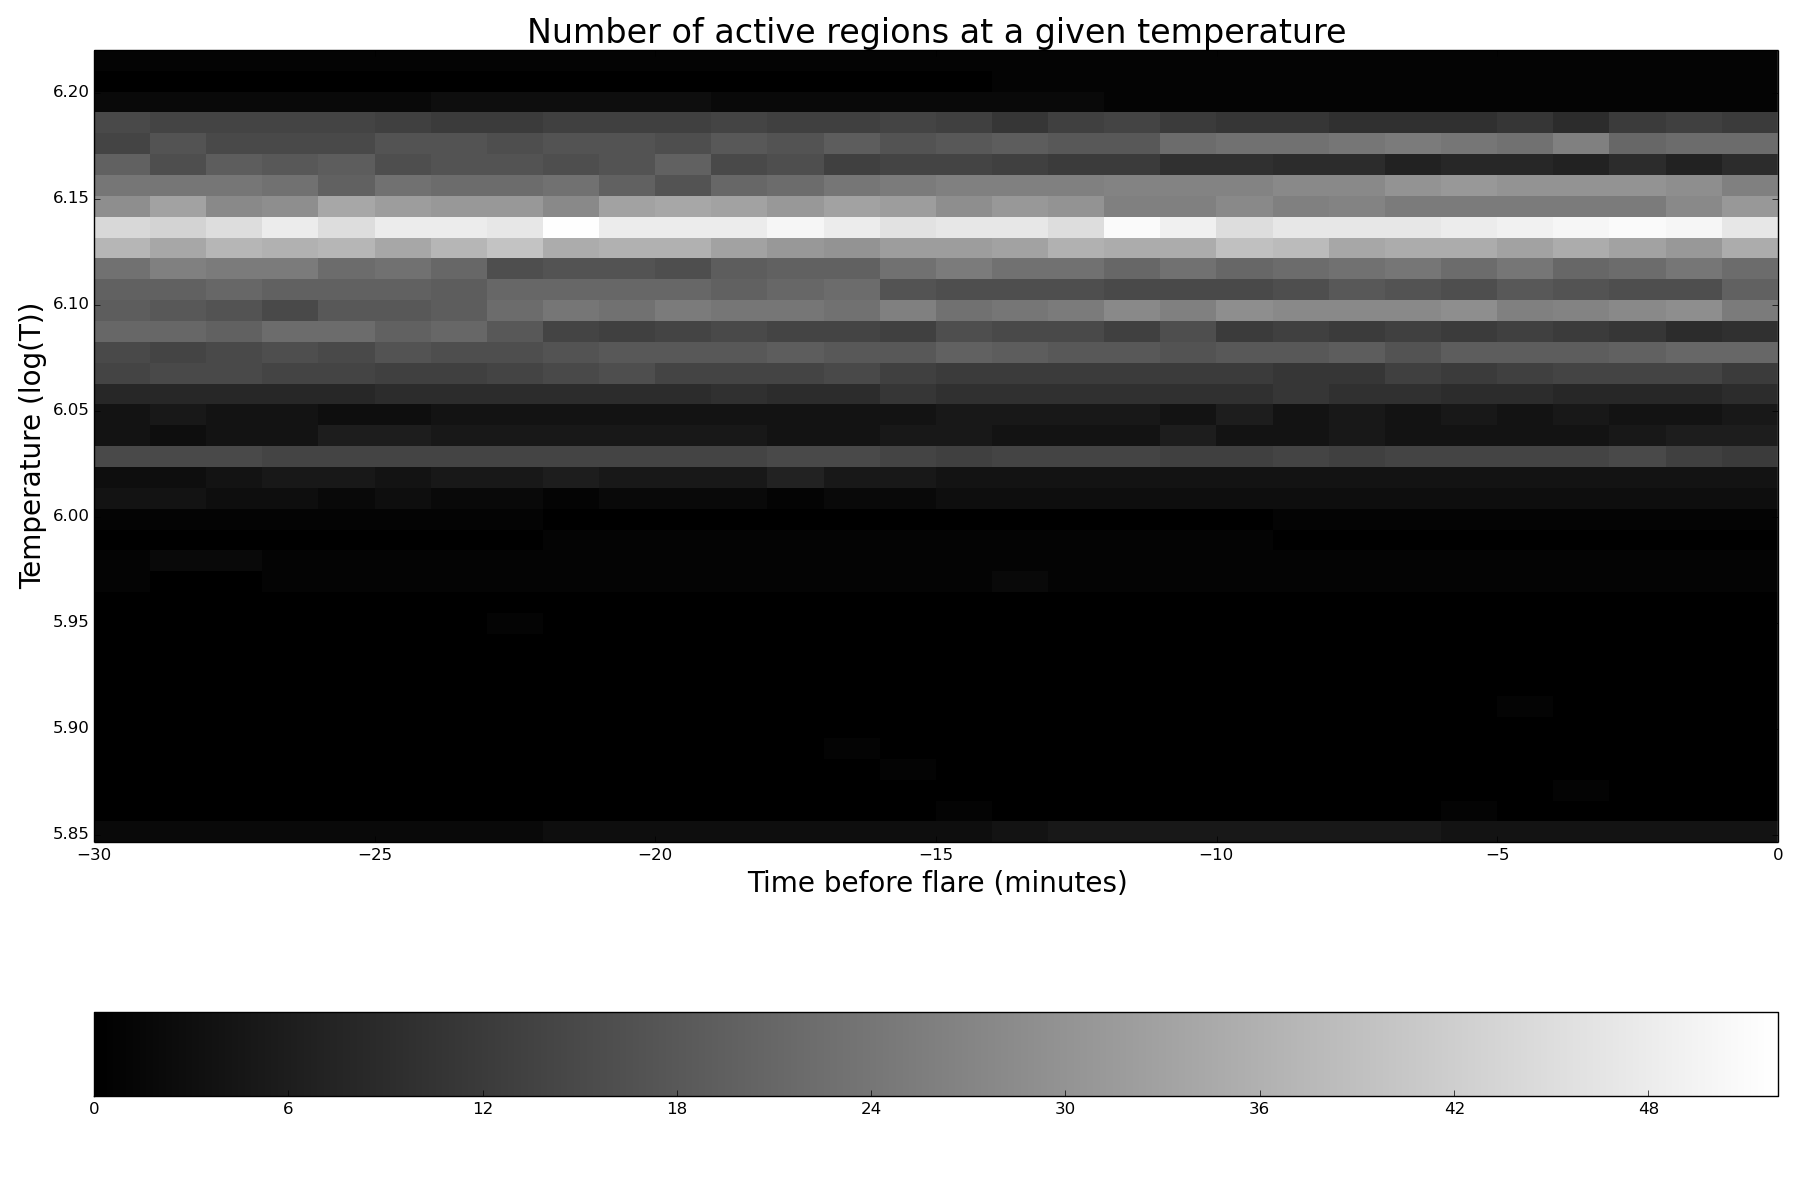
\includegraphics[width=\columnwidth]{tempplotsmean/allars_hist.png}
	\caption{Change in mean temperature of the corresponding active region plotted for each flare as a function of time before the flare began.
		Plots are the same as in Figure \ref{fig:allars_max}.}
	\label{fig:allars_mean}
\end{figure}

\subsection{Flare flux vs temperature}
For each temperature parameter, the value for each flare was plotted on a scatter graph against the peak flux of the flare (Figs. \ref{fig:allflares_max}, \ref{fig:allflares_p95}, \ref{fig:allflares_mean}).
This was done for four times in each case: 30 minutes before the flare start time, 10 minutes before, 1 minute before and at the flare start time.

% Description of plots for maximum
Figure \ref{fig:allflares_max} shows that the maximum temperatures of the ARs studied are closely grouped around a few temperature values.
This remains the case throughout the 30 minutes before the flare, despite the fact that the temperature of many of these active regions rises and falls significantly during this time.
This sudden increase or decrease of temperature is particularly noticeable in the active regions associated with C class flares, as can also be seen in Figure \ref{fig:allars_max}.

% Description of plots for 95
The scatter graphs in Figure \ref{fig:allflares_p95} show that the 95th percentile temperatures of all the active regions were one of only three or four temperautre values, with no apparent dependence on the peak flux of the associated flare. Most of the active regions remain at a constant temperature for most of the period investigated, with only a few displaying any heating or cooling between the times for which the graphs are plotted.

% Description of plots for mean
The mean temperatures of the active regions are more varied than the other parameters, with values ranging between $log(T) \approx 5.95$ and $log(T) \approx 6.25$. 
Most active regions show no clear link between mean temperature and flare flux, with points being distributed quite uniformly on the plot.
However, it may be worth noting that the flare with the highest flux corresponds to an active region with a temperature near the top of the range shown, while some of the weakest flares correspond to the coolest active regions.
The mean temperature of many of the active regions fluxuates somewhat, but any changes are quite small and the overall distribution of the plots remains largely the same.

% Description of plots for p5 and min
As described in Section \ref{sec:temps_v_time}, the 5th-percentile and minimum temperatures showed very little variation, both over time and between active regions.
These values are therefore not shown here since they reveal no useful information.

\begin{figure}
	\centering
		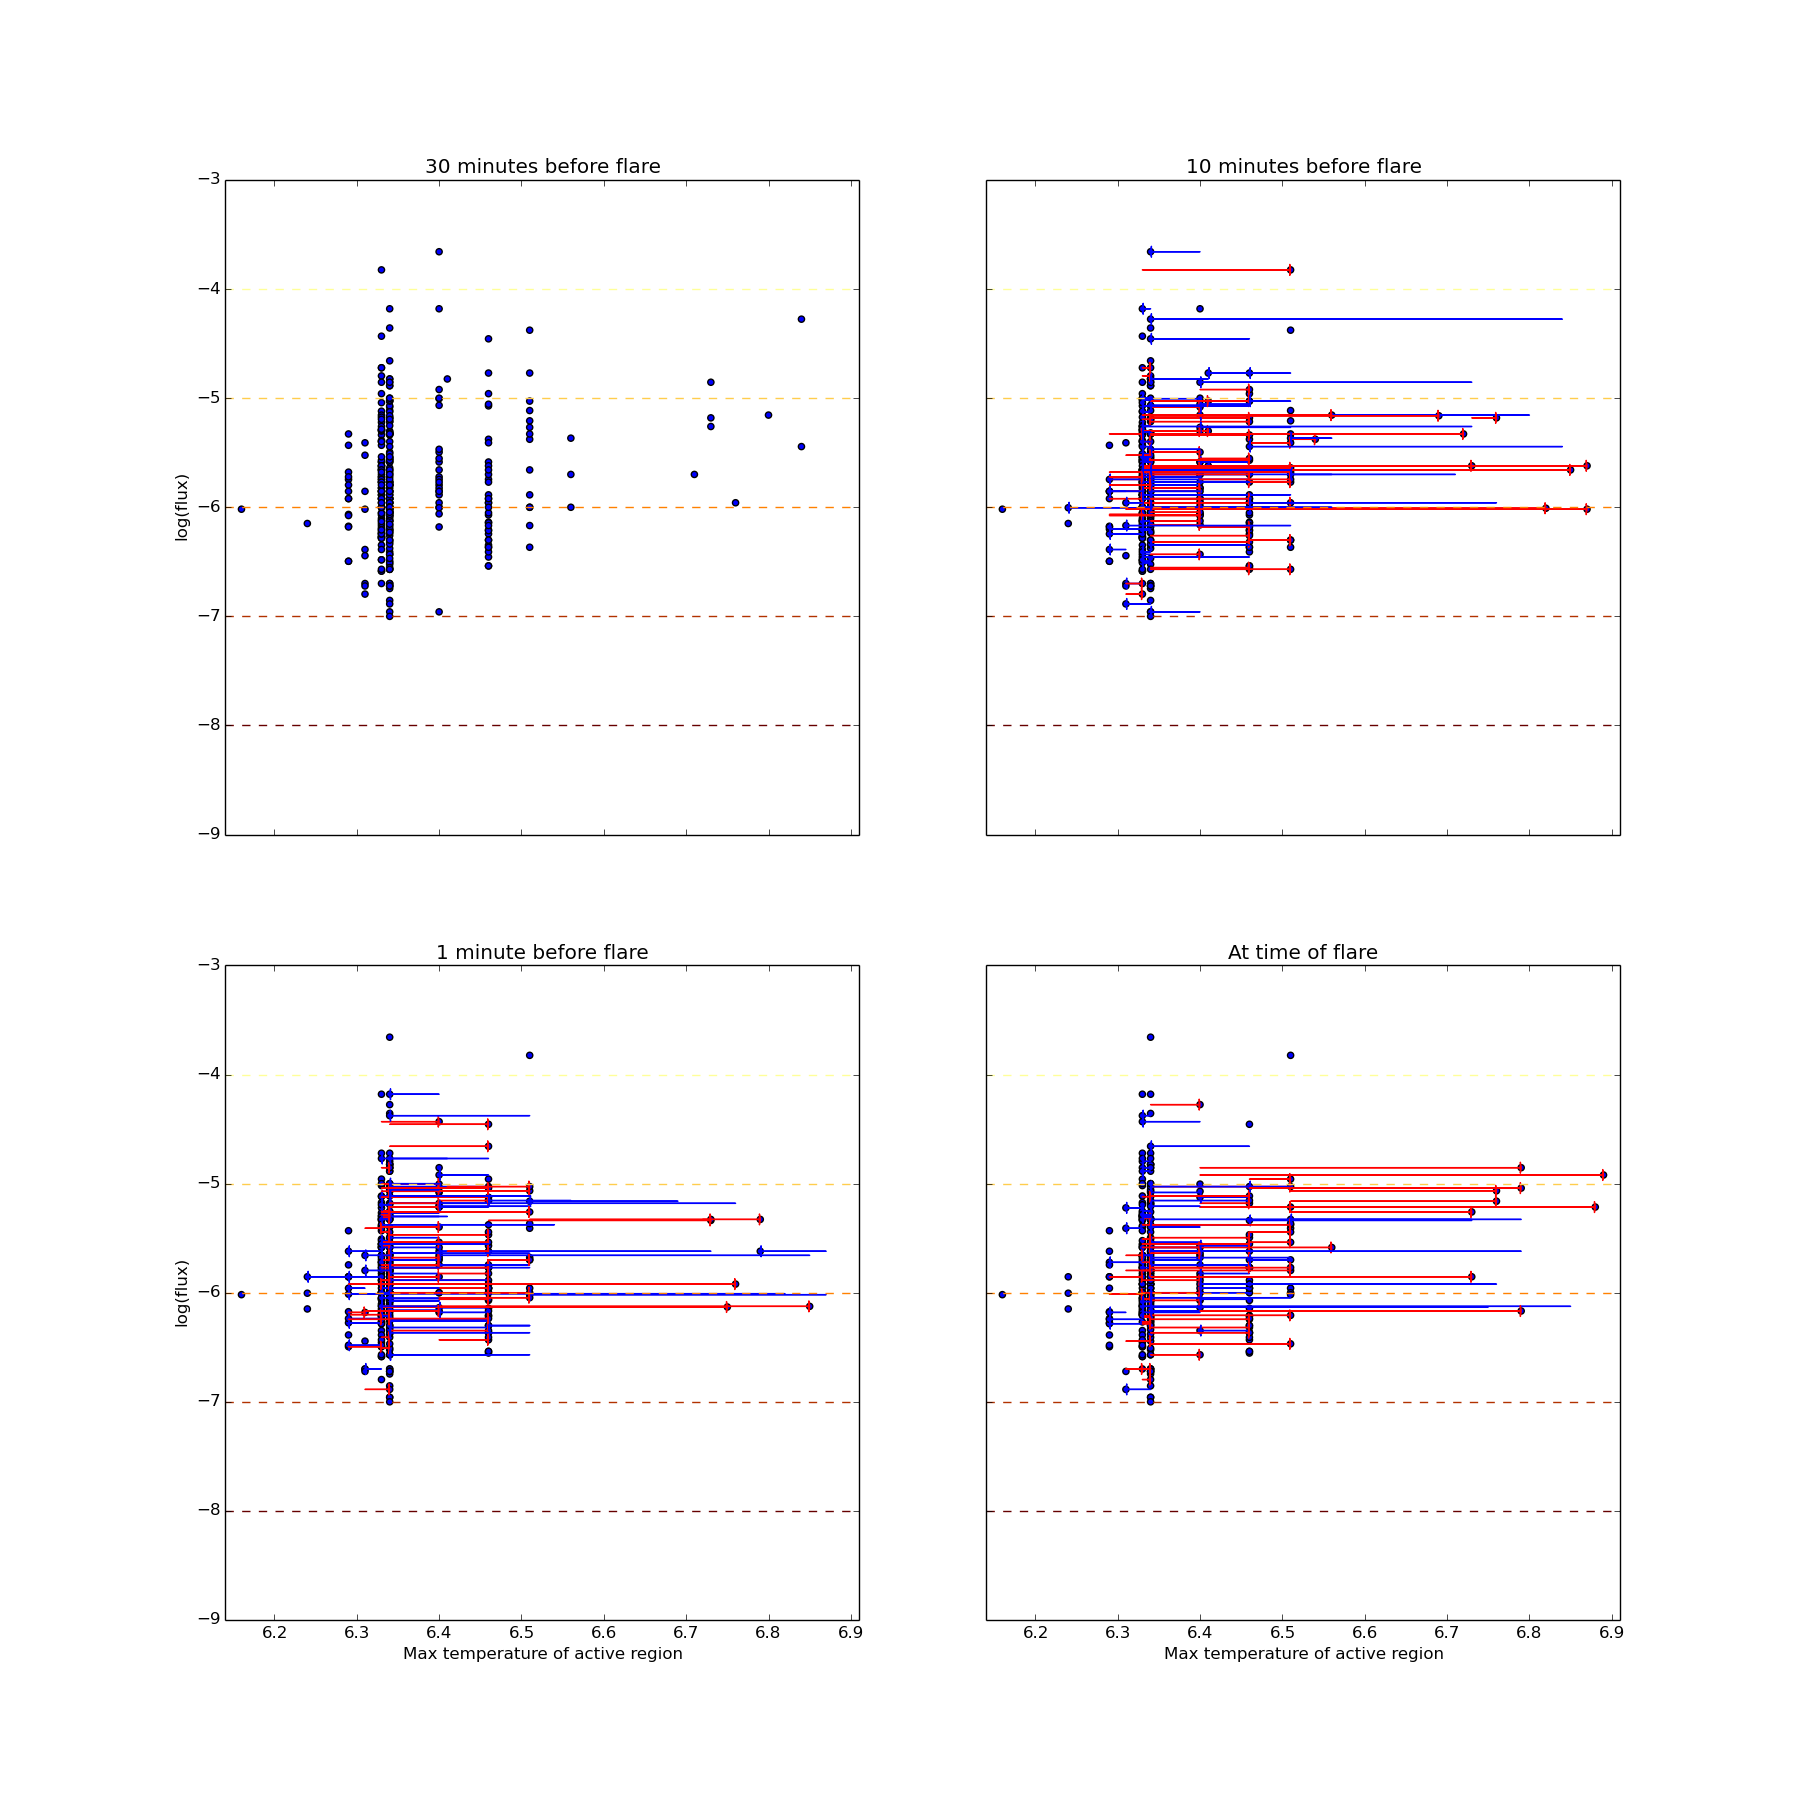
\includegraphics[width=0.9\columnwidth]{tempplotsmax/allflares.png}
	\caption{Scatter graph of flare peak flux against active region maximum temperature for four different times. Top left: 30 minutes before flare start time. Top right: 10 minutes before flare start time. Bottom left: 1 minute before flare start time. Bottom right: flare start time. The red and blue arrows indicate the amount by which the temperature of each active region rose or fell respectively since the time of the previous plot. In each plot the dashed lines indicate the lower X-ray flux thresholds for A, B, C, M and X class flares.}
	\label{fig:allflares_max}
\end{figure}
\begin{figure}
	\centering
		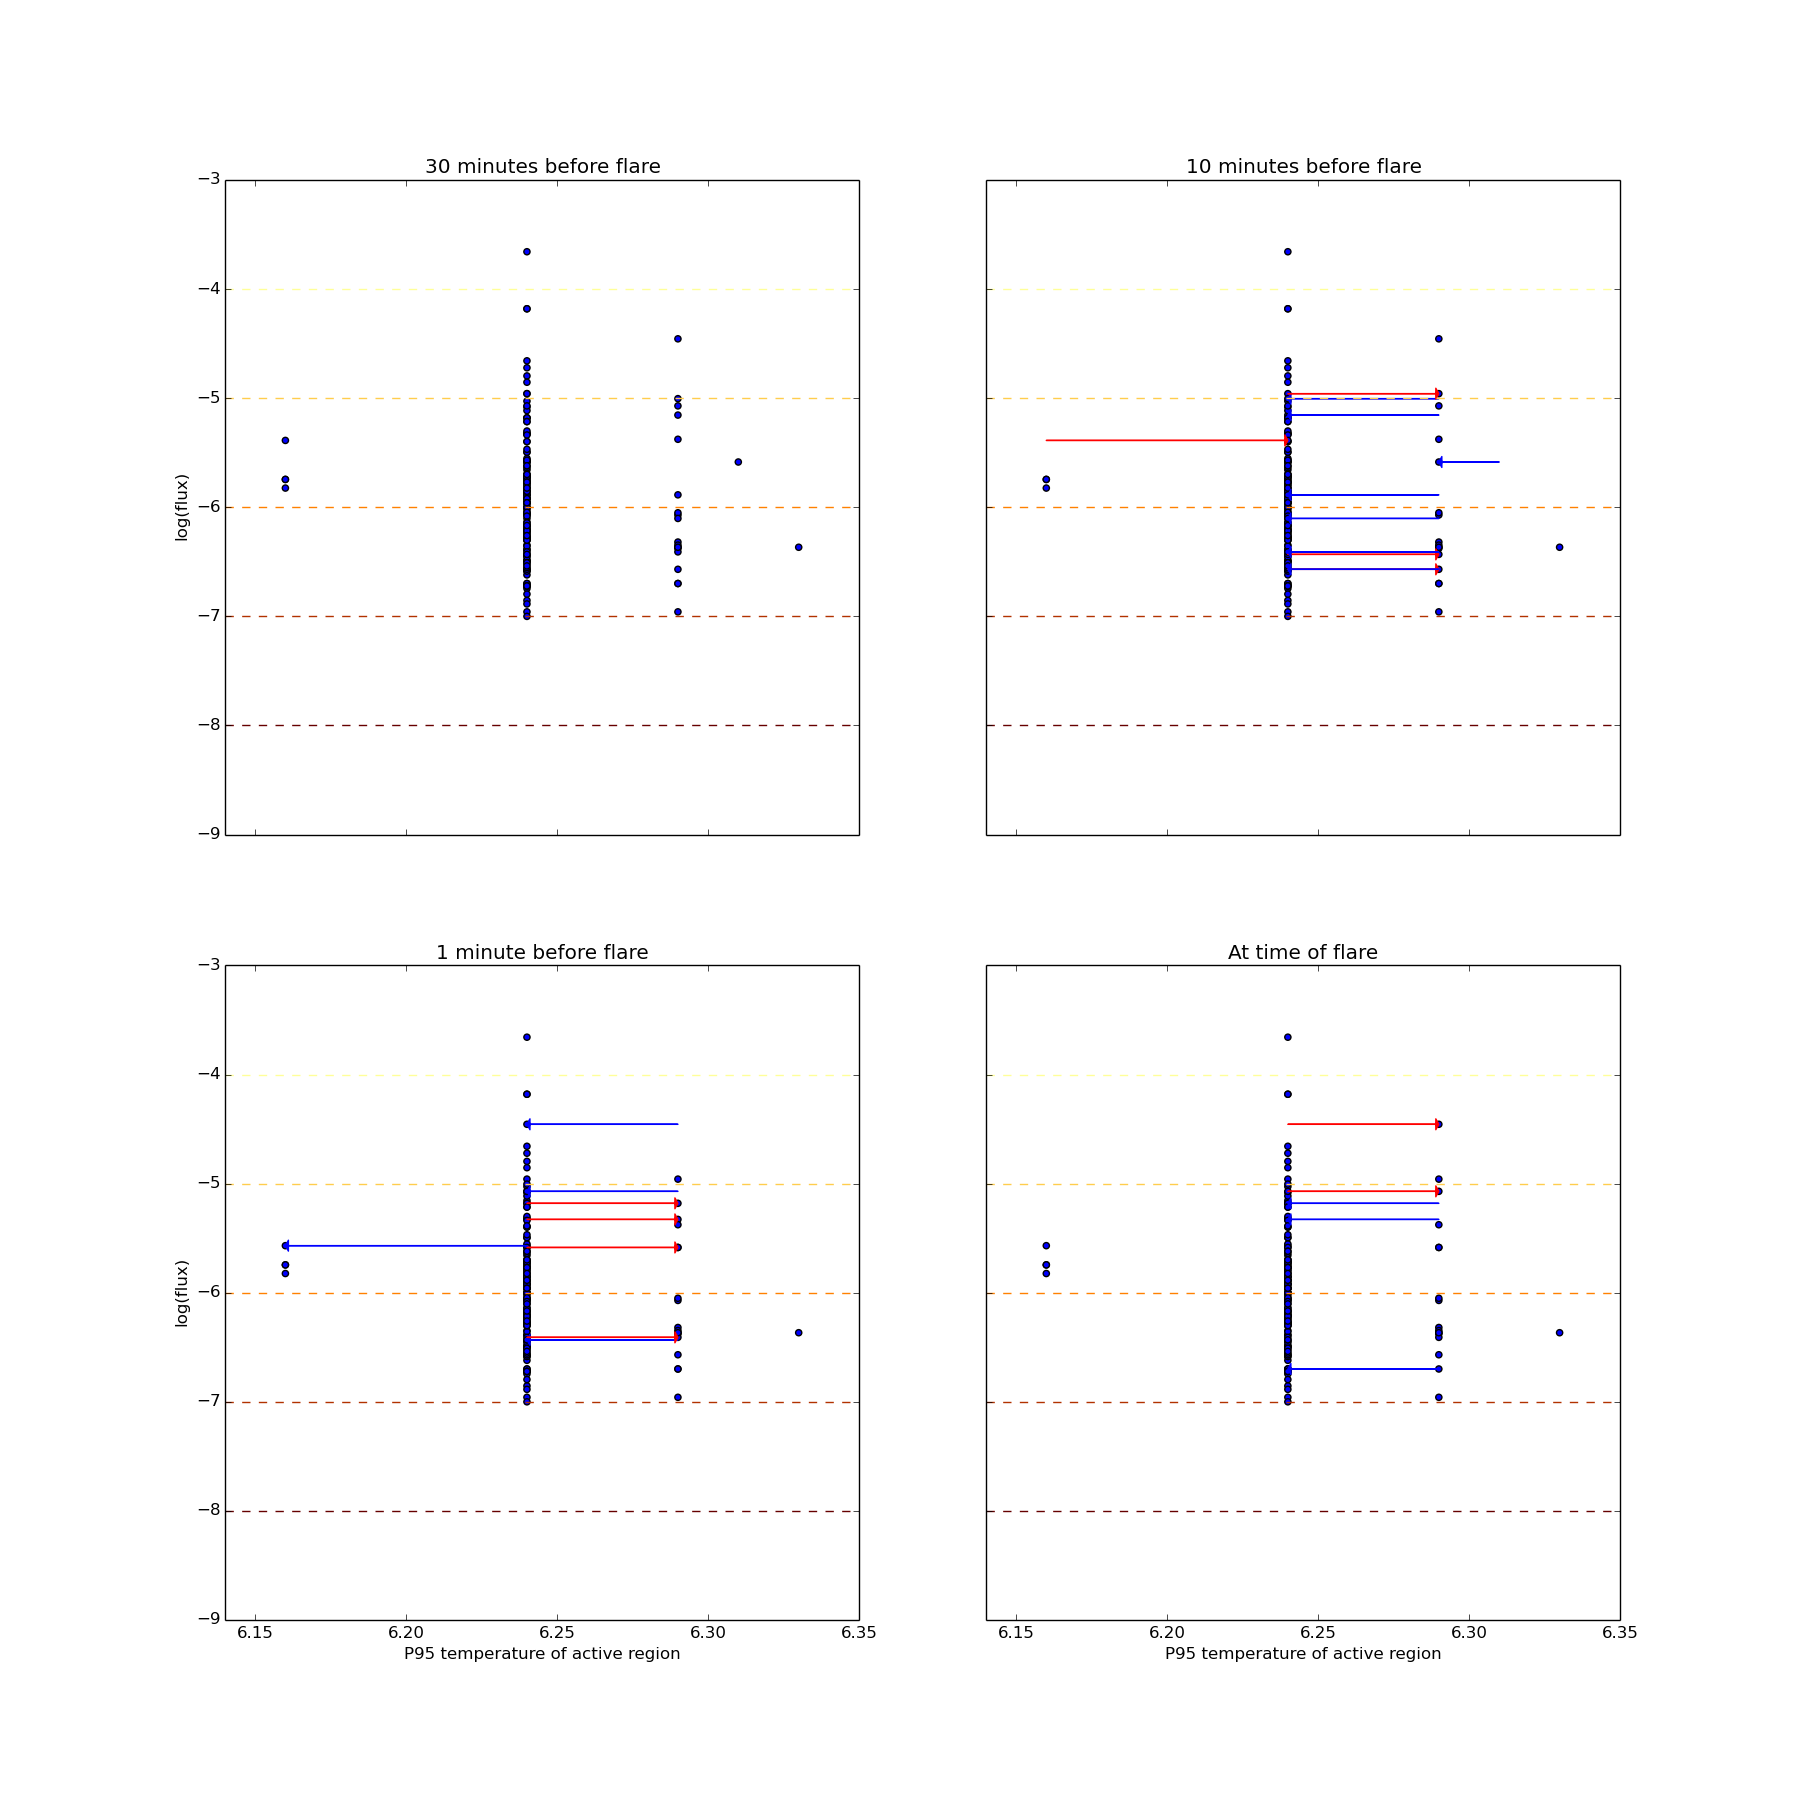
\includegraphics[width=0.9\columnwidth]{tempplots_p95/allflares.png}
	\caption{Scatter graph of flare peak flux against 95th percentile temperature of the corresponding active regions for the same four times as in Figure \ref{fig:allflares_max}.}
	\label{fig:allflares_p95}
\end{figure}
\begin{figure}
	\centering
		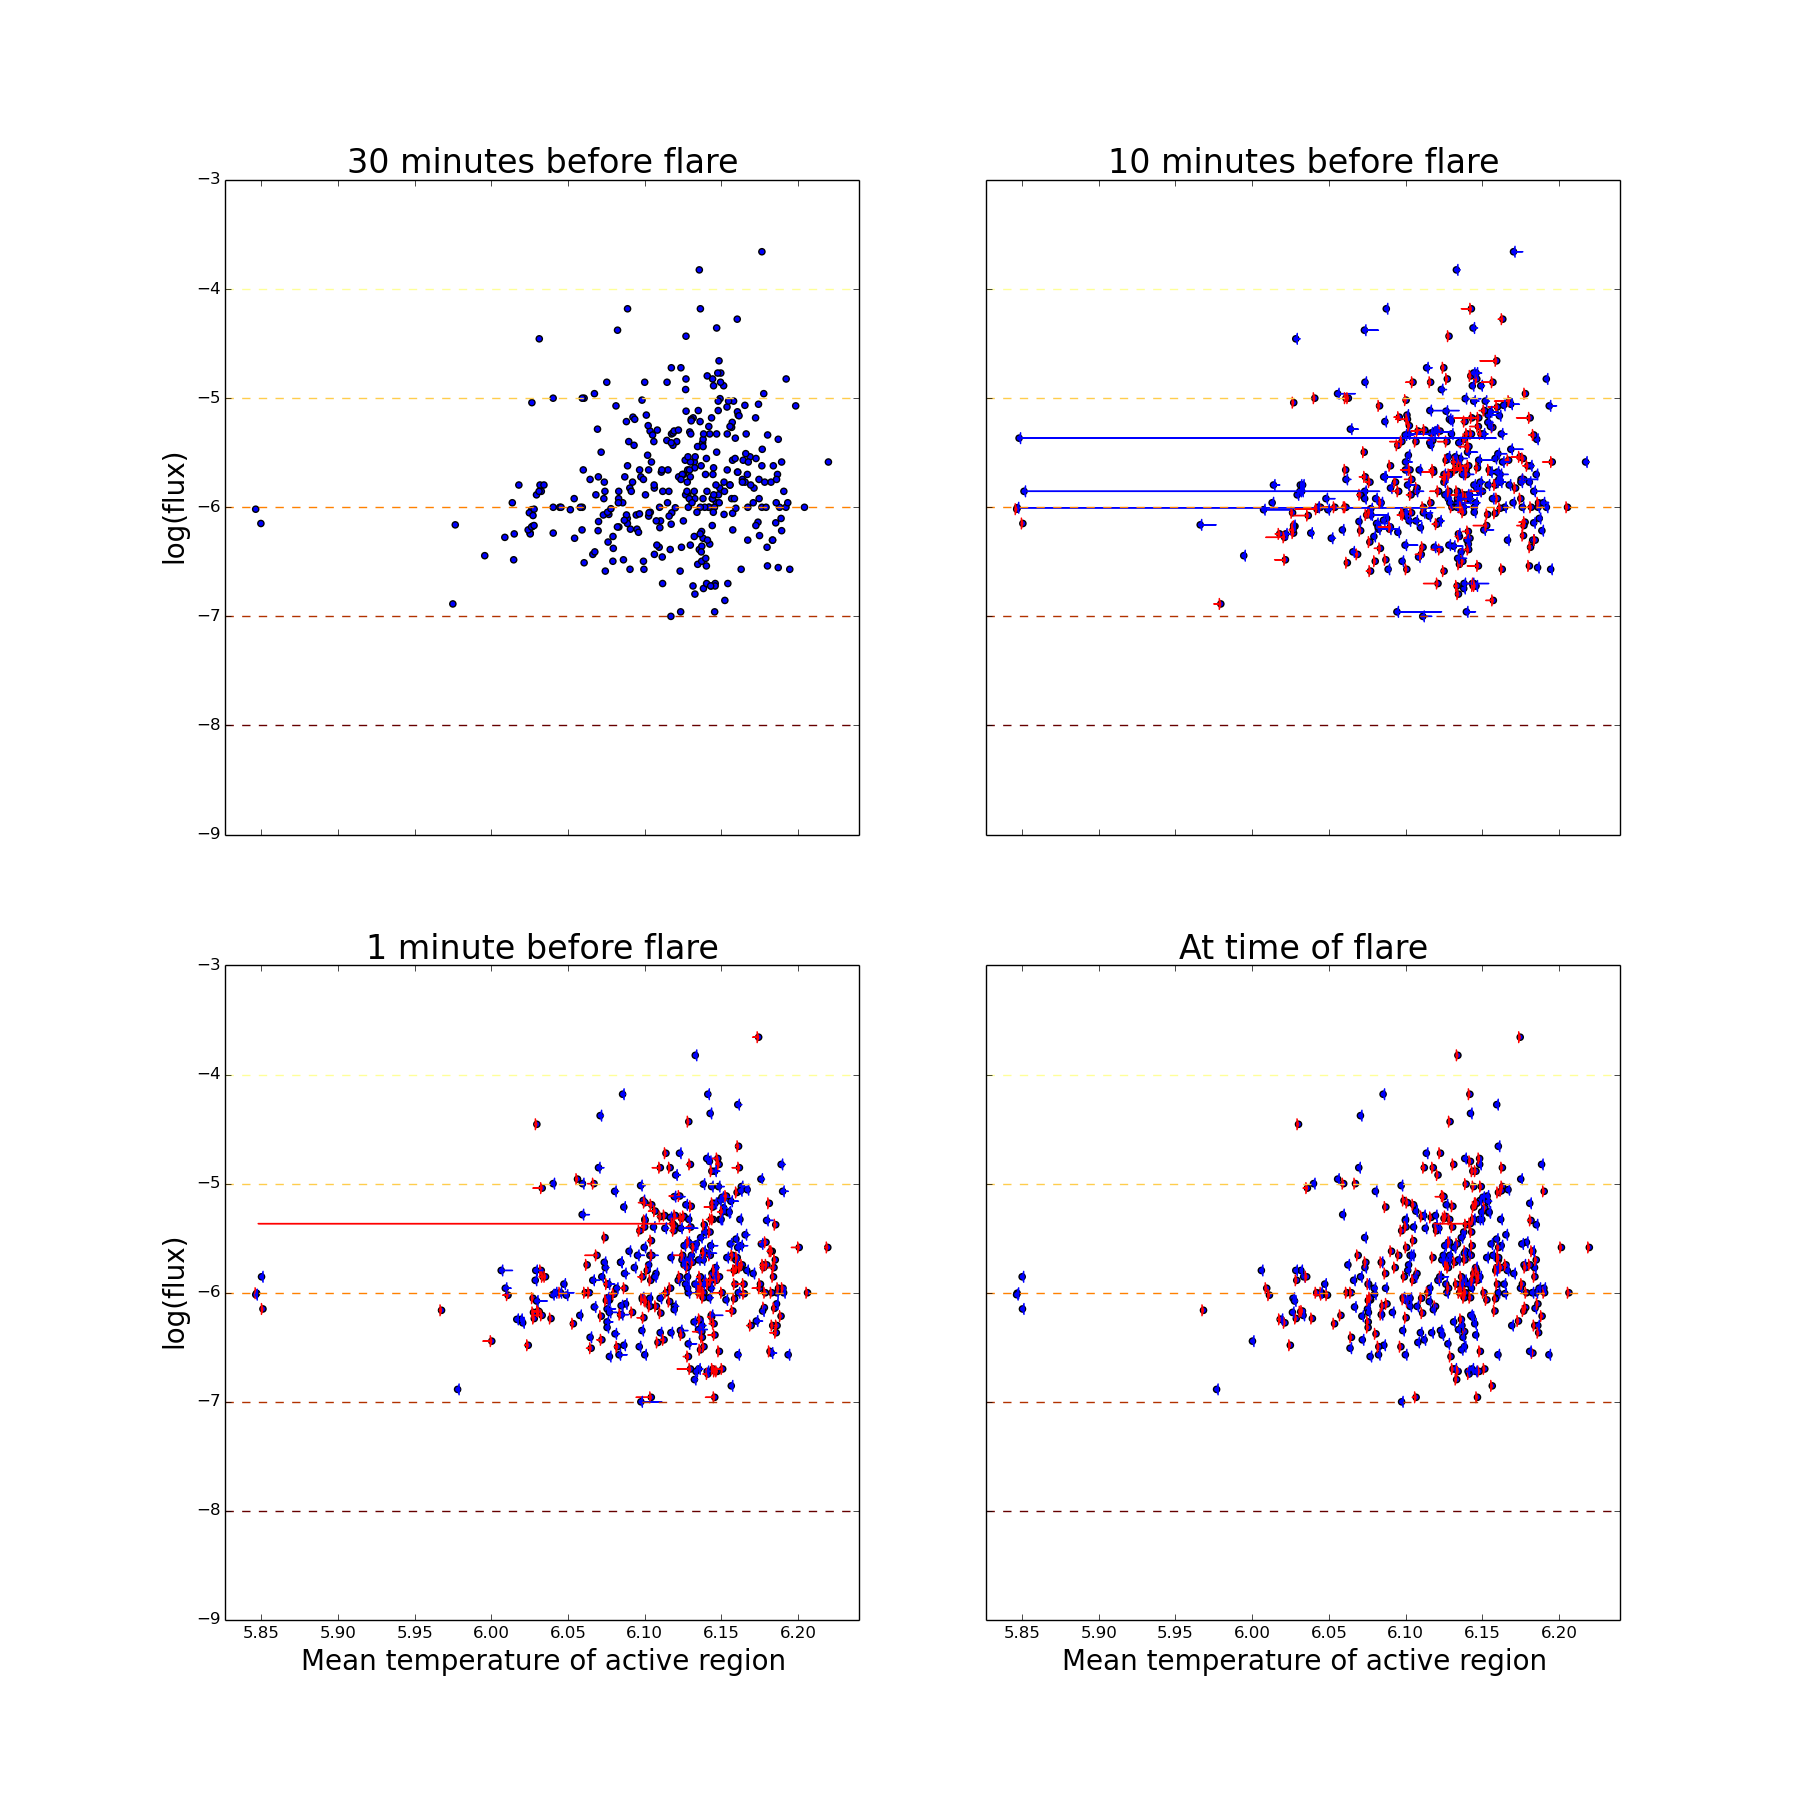
\includegraphics[width=0.9\columnwidth]{tempplotsmean/allflares.png}
	\caption{Scatter graph of flare peak flux against mean temperature of the corresponding active regions for the same four times as in Figure \ref{fig:allflares_max}.}
	\label{fig:allflares_mean}
\end{figure}

%===========================================================================
\section{Discussion and conclusions}
From this study, it appears that there is no clear link between solar flares and the evolution of active region temperatures prior to flaring.
This is probably mostly due to the relatively small number of flares studied - a much larger sample size would have to be used to properly determine any link or lack thereof.
In particular, this study only included a single X class flare, which are the most energetic and the kind we would most wish to predict.
Future works should therefore aim to consider larger flares.
Non-flaring active regions should also be taken into account and compared against the results presented here.
However, this work does demonstrate that it is now possible to study temperature distributions of the corona in high resolution and on short timescales using fast temperature analysis tools such as the one described in \citetalias{Leonard}.

Figures \ref{fig:allars_max} - \ref{fig:allars_mean} show that there is no clear trend in any of the temperature parameters investigated before flares occur.
However, this study only looks at quite a short amount of time before flares; an investigation into longer-term temperature distributions may yield better results.

Similarly, no clear correlation can be seen between peak flare flux and active region temperature, but a much larger sample of flares is needed in order to properly determine whether or not a link exists between the two.
Some of the points on Figure \ref{fig:allflares_mean} do appear to show a rise in temperature with peak flare flux, but the sample size is too small and there are too many other points which do not show such a relation for this to be considered a positive result.

Finally, it is worth remembering that this study only looks at the bulk properties of the active region temperatures.
Any temperature changes leading up to flares may occur on the scale of only a few pixels.
For this reason, the full distribution of temperatures in the active region should be investigated in detail in a future study.

%===========================================================================
\begin{acknowledgements}
	This research has made use of SunPy, an open-source and free community-developed solar data analysis package written in Python \citep{Mumford2013}.
	AIA images and data are courtesy of NASA/SDO and the AIA science team.
\end{acknowledgements}

%===========================================================================
\section*{Annexes}
% Also try and put two sets of columns on a page so it takes up less space
\begin{longtable}{c|c|c}
	\caption{Start times and associated active regions of solar flares studied between 2011/02/01 and 2011/03/31.}\\
		Date and time & GOES class & NOAA Active region \\
		\hline
		\input{tempplotsmean/flarelist.txt}
	\label{tab:flares}
\end{longtable}

%===========================================================================
\bibliography{C:/Users/Drew/Dropbox/Thesis/thesis_refs,C:/Users/Drew/Documents/library}

\end{linenumbers}
\end{document}